%%%%%%%%%%%%%%%%%%%%%%%%%%%%%%%%%%%%%%%%%%%%%%%%%%%%%%%%%%%%%%%%%%%%%%%%%%%%%%%%%%%%%%%%%%%%%
%%									Chapitre 3												%
%%%%%%%%%%%%%%%%%%%%%%%%%%%%%%%%%%%%%%%%%%%%%%%%%%%%%%%%%%%%%%%%%%%%%%%%%%%%%%%%%%%%%%%%%%%%%
\chapter{Implantation du programme}
	\minitoc
	\newpage
%%%%%%%%%%%%%%%%%%%%%%%%%%%%%%%%%%%%%%%%%%%%%%%%%%%%%%%%%%%%%%%%%%%%%%%%%%%%%%%%%%%%%%%%%%%%%
Une application Android est un assemblage de composants liés grâce à un fichier de configuration.
Activite : fenêtre dont il est possible de naviguer, il contient les contextes (lien entre système et autres) pour le gérer on a une liste LIFO:\\
 Les Activités est exends activity \\
Les vue est extend view\\

\section{Cycle de vie d'une activité}
En Android, une activité est une composante de l'application qui représente une seule fenêtre, avec une interface utilisateur, sur l'écran de l'appareil. Chaque activité a un cycle de vie qui décrit son état à différents moments, depuis sa création jusqu'à sa destruction. Le cycle de vie d'une activité est géré par le système Android et suit un ensemble de méthodes spécifiques qui sont appelées à différentes étapes. Voici les principales étapes du cycle de vie d'une activité :
  \begin{itemize}  
    \item[-] \textbf{Création (onCreate()) : } Cette méthode est appelée lorsque l'activité est d'abord créée. C'est généralement l'endroit où vous effectuez l'initialisation de base, telle que l'inflation de la mise en page (layout) et l'initialisation des objets nécessaires.
    \item[-] \textbf{Démarrage (onStart()) :} Après la création, l'activité passe à l'état de démarrage. À ce stade, l'activité devient visible à l'utilisateur, mais elle n'est pas encore interactive.
    \item[-] \textbf{Reprise (onResume()) :}  L'activité est maintenant en état de reprise. C'est le moment où elle devient active et l'utilisateur peut interagir avec elle. Cette méthode est également le meilleur endroit pour enregistrer des gestionnaires d'événements ou des mises à jour de l'interface utilisateur.
    \item[-] \textbf{Mise en arrière-plan (onPause()) :}  L'activité est en cours d'entrée en arrière-plan. Elle reste visible, mais elle n'accepte généralement plus d'entrées de l'utilisateur. À ce stade, vous pouvez enregistrer les données nécessaires pour restaurer l'état de l'activité si nécessaire.
    \item[-] \textbf{ Arrêt (onStop()) :} L'activité n'est plus visible à l'utilisateur. À ce stade, elle est en cours d'arrêt et peut être arrêtée par le système pour libérer des ressources.
    \item[-] \textbf{Redémarrage (onRestart()) :}  L'activité est en cours de redémarrage après avoir été arrêtée. Elle est sur le point de revenir à l'état de reprise.
    \item[-] \textbf{ Démarrage (onStart()) et Reprise (onResume()) :} Si l'activité passe par un redémarrage, elle retourne ensuite à l'état de démarrage et de reprise.
    \item[-] \textbf{Arrêt (onStop()) :}  Si l'activité n'est plus visible à l'utilisateur (par exemple, si une autre activité a été lancée), elle passe à l'état d'arrêt.
    \item[-] \textbf{Destruction (onDestroy()) : } L'activité est détruite. Cela se produit lorsque l'activité est explicitement fermée par l'utilisateur ou lorsque le système décide de libérer des ressources. C'est le dernier point du cycle de vie de l'activité.

\end{itemize}
%%%%%%%%%%%%%%image activity
	\begin{figure}[!h]
    	\center
    		\includegraphics[width=0.8\textwidth]{image/cycle}
   		\caption{Cycle de vie d'une activité}
    	\label{Cycle de vie d'une activité}
	\end{figure}
\section{Les intentes}
Pour communiquer c’est-à-dire faire circuler des messages d’une application a une autre ou à l'intérieur d'une même application il faut savoir plusieur chose.il y Les agents qui sont chargés de ce mécanisme d'échange s'appellent les intents. Ce mécanisme est tellement important qu'Android lui-même l'utilise massivement en interne.\\
Un intent est en fait un objet qui contient plusieurs champs, représentés à la figure suivante
%%%%%%%%%%%%%image intent
\begin{figure}[!h]
    	\center
    		\includegraphics[width=0.3\textwidth]{image/intent.png}
   		\caption{Une intent}
    	\label{Une intent}
	\end{figure}
\section{Modelisation du programme}
\subsection{Organigrame pour agriculture biodynamique }
L'agriculture biodynamique est bien plus qu'une simple méthode de culture ; c'est un système holistique qui intègre des pratiques agricoles traditionnelles avec une compréhension profonde des cycles naturels, y compris le cycle lunaire. Voici comment ce système fonctionne en harmonie avec les phases de la lune pour produire des cultures saines et durables.
L'objectif principal de cet organigramme est de faciliter la décision quant aux plantes à planter à des dates spécifiques, en se basant sur la phase lunaire correspondante. Le processus commence par la saisie d'une date précise, suivie de l'identification de la phase lunaire associée à cette date. Ensuite, en fonction de cette phase lunaire, l'organigramme détermine le type de plante le plus approprié à planter : feuille, fleur, racine ou bourgeon. Cette approche permet une gestion plus efficace des cultures en tenant compte des influences lunaires sur la croissance des plantes, contribuant ainsi à optimiser les rendements agricoles tout en respectant les cycles naturels.
\begin{itemize} 
\item[-] \textbf{Initialisation des paramètres :}\\
Avant de commencer toute activité agricole, les agriculteurs biodynamiques prennent en compte le calendrier lunaire pour déterminer les différentes phases de la lune, y compris la nouvelle lune, le premier quartier, la pleine lune et le dernier quartier.
\item[-] \textbf{Planification des activités agricoles :}\\
 En se basant sur les principes de la biodynamique, un calendrier des activités agricoles est établi, en tenant compte des phases de la lune. Pendant la période de la nouvelle lune jusqu'au premier quartier, les activités favorisent la croissance des parties aériennes des plantes. Entre le premier quartier et la pleine lune, les activités sont axées sur la floraison et la fructification. Pendant la période entre la pleine lune et le dernier quartier, l'accent est mis sur la croissance des racines et la consolidation des fruits. Enfin, entre le dernier quartier et la nouvelle lune, les activités se concentrent sur la préparation du sol, la gestion des mauvaises herbes et la récolte des cultures à maturité.
\item[-] \textbf{ Application des préparations biodynamiques :}\\
Pendant les périodes propices du cycle lunaire, des préparations biodynamiques spécifiques sont appliquées au sol et aux cultures, en tenant compte des recommandations spécifiques pour chaque phase de la lune. Ces préparations sont conçues pour dynamiser le sol et favoriser la santé des plantes.
\end{itemize}
\begin{figure}[H]
    	\center
    		\includegraphics[width=1\textwidth]{image/org}
   		\caption{Organigramme de calcul de phase de la lune}
    	\label{Organigramme de calcul de phase de la lune}
	\end{figure}
\subsection{Diagramme de cas d'utilisation}
Il permet la visualisation des interactions entre objets du système La structure d’une opération est découpé en actions. C’est un des moyens de représenter les besoins à couvrir.\\
\begin{figure}[!h]
    	\center
    		\includegraphics[width=1\textwidth]{image/diagrame2/Diagramme_utilisation.jpg}
   		\caption{Diagramme de cas d'utilisation}
    	\label{Diagramme de cas d'utilisation}
	\end{figure}

Le système de gestion de plantes potagères offre une plateforme complète pour répondre aux besoins variés des utilisateurs impliqués dans la culture et la gestion des plantes. Les jardiniers, qui sont responsables de l'entretien quotidien et de la croissance des plantes, peuvent utiliser le système pour planifier et suivre les tâches telles que la plantation, l'arrosage, la fertilisation et la récolte des légumes.

Les gestionnaires, en charge de superviser l'ensemble du processus de gestion des plantes, ont la possibilité de gérer les utilisateurs en ajoutant, modifiant ou supprimant des comptes selon les besoins de l'équipe de jardinage. Ils peuvent également gérer les plantes en ajoutant de nouvelles espèces au catalogue, en modifiant les détails des plantes existantes et en supprimant celles qui ne sont plus cultivées.

Les experts en botanique, qui fournissent des conseils spécialisés sur les soins des plantes, peuvent utiliser le système pour consulter les informations détaillées sur chaque espèce de plante, y compris leurs besoins en lumière, en eau et en nutriments, ainsi que les meilleures pratiques de culture.

Ces activités sont soutenues par des inclusions telles que l'affichage d'informations pertinentes sur les spécifications des plantes, le calcul précis des quantités d'eau et de nutriments nécessaires pour chaque plante, et la possibilité d'effectuer des opérations CRUD complètes pour gérer les données de manière efficace.

Le système démarre dès qu'un utilisateur se connecte, offrant la possibilité de sélectionner une date spécifique pour planifier des tâches de jardinage via un calendrier interactif intégré. Une fois dans le menu Calendrier, l'utilisateur peut choisir une date et lancer un calcul pour déterminer les différentes phases lunaires associées à cette date. Il peut également créer et gérer un potager, en ajoutant de nouvelles plantes, en modifiant les détails des plantes existantes et en supprimant celles qui ne sont plus cultivées.

Enfin, l'option de quitter le système est disponible pour permettre aux utilisateurs de terminer leurs tâches et de quitter l'interface en toute simplicité une fois qu'ils ont accompli leurs actions.
\subsection{Diagramme de classes}
Le diagramme de classe est une représentation visuelle de la structure des données du système, organisée en classes et en relations entre ces classes. Nous avons mis en place plusieurs classes dans notre programme afin de suivre le modèle MVC (Modèle-Vue-Contrôleur). Ce modèle permet de séparer les différentes responsabilités de l'application : le modèle pour la manipulation des données, la vue pour l'affichage des informations à l'utilisateur, et le contrôleur pour la gestion des interactions et la coordination entre le modèle et la vue. Cette approche de conception nous permet de mieux organiser notre code et de faciliter la maintenance et l'évolution du système.\\ 
\begin{itemize} 
\item[-] \textbf{classe principale : }\\
La classe principale de notre application est la classe Main. Elle constitue le point d'entrée initial de notre programme et représente la première interaction entre l'utilisateur et l'application. Cette classe gère l'initialisation de l'application et coordonne les différentes fonctionnalités en interagissant avec l'utilisateur via l'interface utilisateur ou d'autres systèmes. En tant que point de départ de l'application, la classe Main est essentielle pour orchestrer le flux de contrôle et faciliter la communication entre l'utilisateur et le système, assurant ainsi une expérience utilisateur fluide et cohérente.\\	
\begin{figure}[!h]
    	\center
    		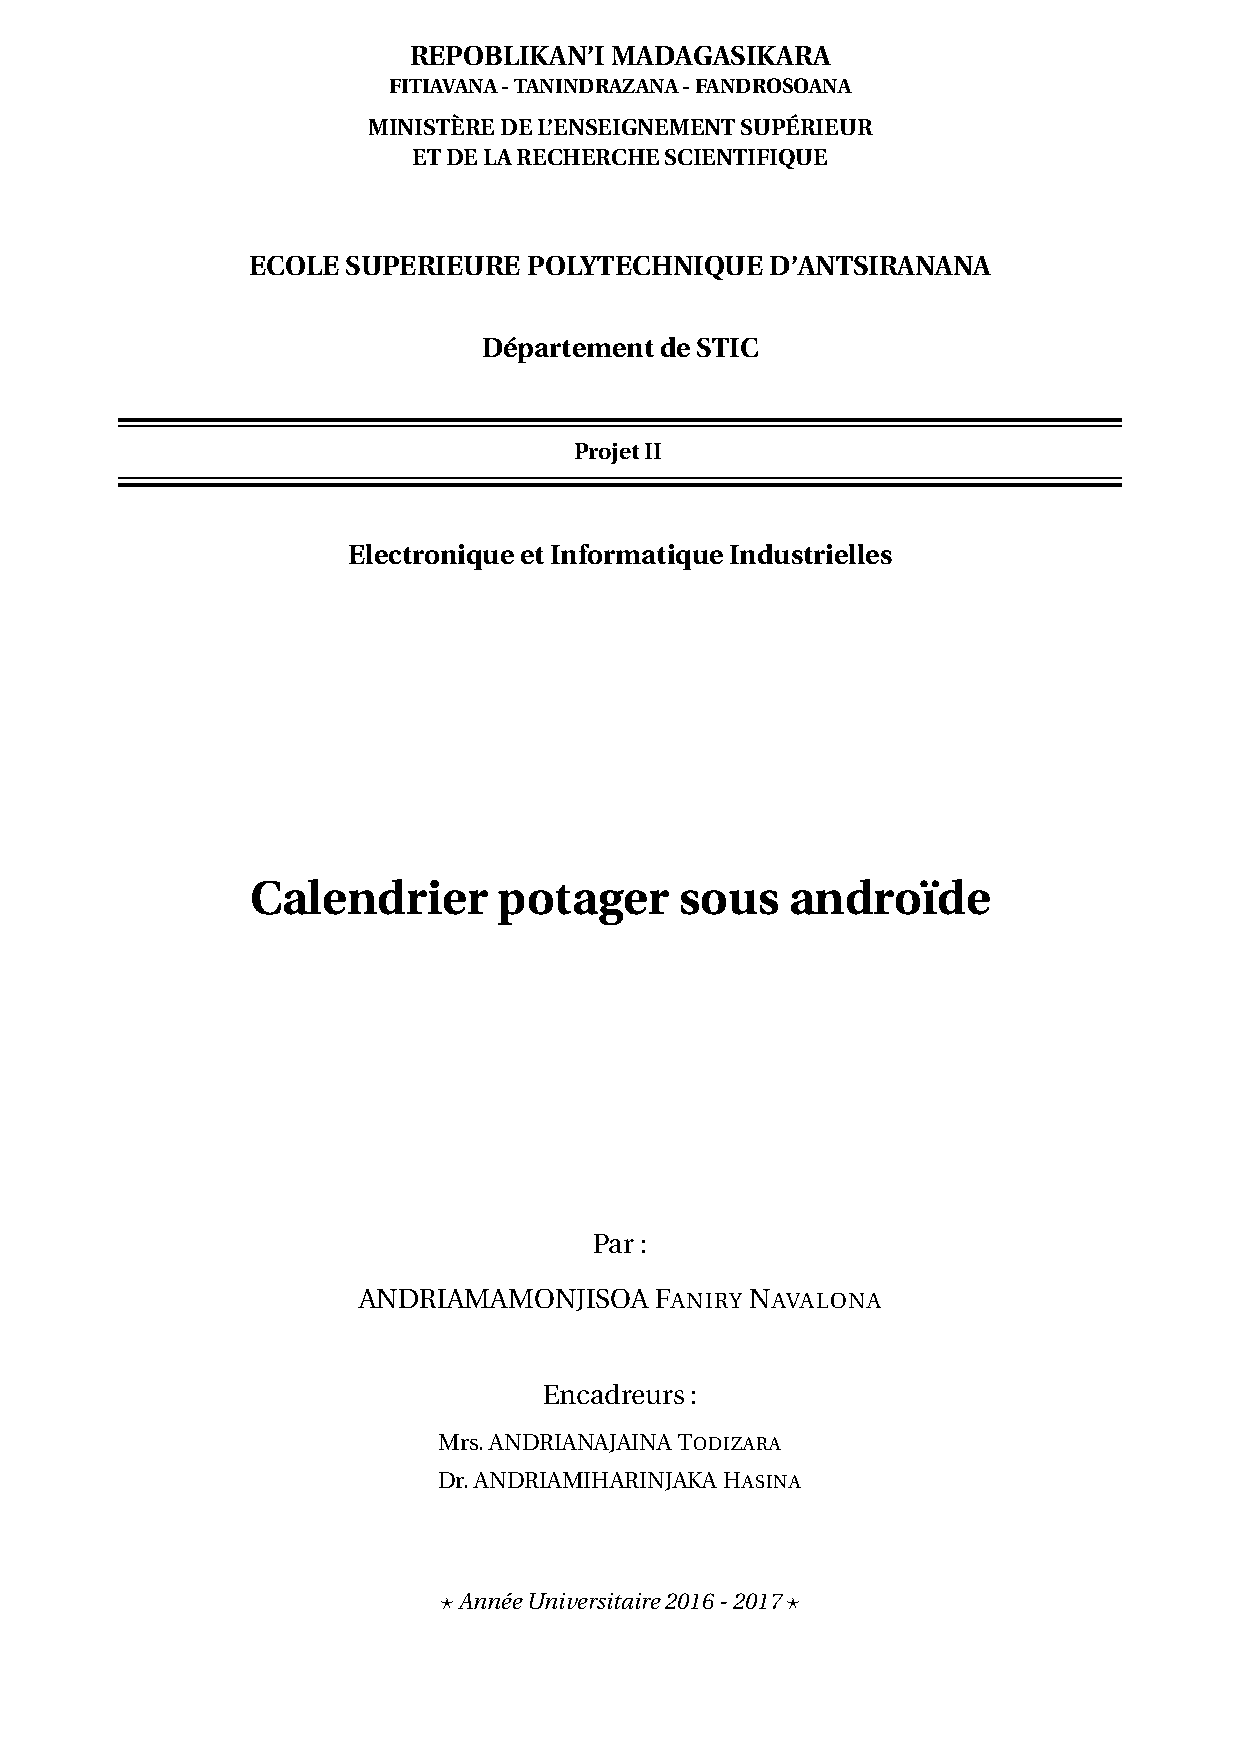
\includegraphics[width=0.4\textwidth]{image/diagrame2/Main.jpg}
   		\caption{Diagramme de classes main}
    	\label{Diagramme de classes}
	\end{figure}\\

\item[-] \textbf{La classe Controller base de données: }\\
La classe Controller Base De Donnees représente le contrôleur dans notre application. Elle agit comme un intermédiaire entre la vue et le modèle, facilitant la communication entre l'utilisateur et la base de données. Cette classe gère les requêtes et les actions de l'utilisateur, puis transmet ces informations au modèle pour effectuer les opérations correspondantes sur la base de données. Le modèle, quant à lui, est une classe de gestion de base de données qui permet d'effectuer des opérations telles que l'ajout, la mise à jour et la suppression de données dans la base de données. Il agit comme une interface entre l'application et la base de données, garantissant une manipulation efficace et sécurisée des données.\\
\begin{figure}[!h]
    	\center
    		\includegraphics[width=0.4\textwidth]{image/diagrame2/Model.jpg}
   		\caption{Diagramme de classes Model}
    	\label{Diagramme de classes Model}
	\end{figure}\\
\item[-] \textbf{La classe type View : }\\
La classe type View représente la vue dans notre application. Le diagramme de classe de la liste de potager sert à afficher les listes de potagers que l’on peut cultiver avec une date sélectionnée. À l'aide de l'objet ListView, cette classe gère précisément une liste. Une fois qu'un élément est sélectionné, il  est enregistré\\
interface entre l'application et la base de données, garantissant une manipulation efficace et sécurisée des données.\\
	\begin{figure}[!h]
    	\center
    		\includegraphics[width=0.4\textwidth]{image/diagrame2/Liste_potagerActivity.jpg}
   		\caption{Diagramme de classe de liste de potager}
    	\label{Diagramme de classe de liste de potager}
	\end{figure}\\
\end{itemize}
\subsection{Diagramme de séquence}
Le diagramme de séquence, outil crucial en conception logicielle, offre une représentation visuelle des interactions temporelles entre les différents objets impliqués dans la réalisation d’une interface homme-machine. Il joue un rôle essentiel en permettant de décrire de manière détaillée les scénarios d'utilisation, chaque cas d'utilisation étant accompagné d'un scénario décrivant chronologiquement les actions d'un acteur sur le système.\\
 Ce diagramme offre une compréhension approfondie à la fois sur la nature des informations échangées entre les objets et sur l’ordonnancement précis des événements qui se produisent lors de l'exécution du scénario.\\
	\begin{figure}[H]
    	\center
    		\includegraphics[width=1\textwidth]{image/diagrame2/Diagramme_séquencevao.jpg}
   		\caption{Diagramme de séquence génerale}
    	\label{Diagramme de séquence génerale}
	\end{figure}
	
	Dans le contexte de la séquence de gestion d'un nouveau jardin implique l'interaction de l'utilisateur avec l'interface logicielle pour créer et gérer un nouvel espace de jardinage. Cette séquence comprend plusieurs étapes pour faciliter la création et la gestion efficace du jardin :
Tout d'abord, l'utilisateur lance l'application de gestion de jardin potager et sélectionne l'option pour créer un nouveau jardin. 
Ensuite, une fois que les détails du jardin ont été enregistrés, l'utilisateur est dirigé vers la fonctionnalité qui lui permet d'explorer une liste de plantes disponibles pour la culture dans son jardin. \\
L'utilisateur peut ensuite parcourir cette liste de plantes et sélectionner. \\
Une fois que l'utilisateur a choisi les plantes à cultiver, l'interface lui permet de les ajouter à son jardin virtuel. \\
	\begin{figure}[!h]
    	\center
    		\includegraphics[width=1\textwidth]{image/diagrame2/Gerer_potager.jpg}
   		\caption{Diagramme de séquence gestion de nouveau jardin}
    	\label{Diagramme de séquence gestion de nouveau jardin}
	\end{figure}
	
	\begin{figure}[!h]
    	\center
    		\includegraphics[width=1\textwidth]{image/diagrame2/Gerer_potager2.jpg}
   		\caption{Diagramme de séquence gestion de jardin enregistrer}
    	\label{Diagramme de séquence gestion de jardin enregistrer}
	\end{figure}
	Le diagramme de séquence relatif au calcul de la phase lunaire offre une représentation détaillée des interactions entre les différents composants logiciels impliqués dans le processus de détermination de la phase actuelle de la lune. Ce processus commence généralement par l'acquisition de la date choisie par l'utilisateur. Ensuite, le logiciel effectue des calculs pour déterminer la position actuelle de la lune dans son orbite autour de la Terre, en utilisant des algorithmes astronomiques appropriés.\\
Une fois que la position de la lune est déterminée, le logiciel identifie la phase lunaire correspondante, comme la nouvelle lune, le premier quartier, la pleine lune ou le dernier quartier. \\
	\begin{figure}[!h]
    	\center
    		\includegraphics[width=1\textwidth]{image/diagrame2/calcul_phase_lunaire.jpg}
   		\caption{Diagramme de séquence calcul du phase lunaire}
    	\label{Diagramme de séquence calcul du phase lunaire}
	\end{figure}
\subsection{Diagramme d'activités}
Il permet la représentation du comportement entre les objets d’une même classe en termes d'états et de transitions d'états, qui est lié à celui du diagramme de séquence. Cette représentation permet de décrire comment un objet passe d'un état à un autre en réponse à des événements ou des actions. Contrairement au diagramme de séquence qui se concentre sur les interactions entre les objets à un moment donné, le diagramme d'états-transitions montre comment le comportement d'un objet peut changer au fil du temps, en fonction de son état interne et des stimuli externes, comme ici :\\
\begin{figure}[!h]
    	\center
%    		\includegraphics[width=1\textwidth]{image/diagrame2/Diagramme_activités2.jpg}
   		\caption{Diagramme d'état génerale}
    	\label{Diagramme d'état génerale}
	\end{figure}
	Le cycle de vie de l'activité de gestion d'un nouveau jardin englobe plusieurs étapes clés, depuis sa création initiale jusqu'à la gestion quotidienne des données. Tout d'abord, la phase de création implique la mise en place initiale du jardin dans le logiciel de gestion, où l'utilisateur peut saisir des informations telles que l'emplacement, les dimensions, et d'autres détails pertinents pour définir l'espace de jardinage.
Ensuite, lors de la phase d'ajout de données, l'utilisateur peut enrichir le jardin en entrant des informations supplémentaires telles que les types de plantes prévues pour la culture, les dates de plantation, les méthodes de culture envisagées, et d'autres détails utiles. Cette étape permet de personnaliser davantage la planification et la gestion du jardin, en tenant compte des préférences et des besoins spécifiques de l'utilisateur.
	\begin{figure}[!h]
    	\center
    		\includegraphics[width=0.3\textwidth]{image/diagrame2/gerer_potager_new.jpg}
   		\caption{Diagramme d'état gestion nouveau jardin}
    	\label{Diagramme d'état  gestion nouveau jardin}
	\end{figure}
	Ensuite, lors de la phase d'ajout de données, l'utilisateur peut enrichir le jardin en entrant des informations supplémentaires telles que les types de plantes prévues pour la culture, les dates de plantation,et d'autres détails utiles. Cette étape permet de personnaliser davantage la planification et la gestion du jardin, en tenant compte des préférences et des besoins spécifiques de l'utilisateur.
Enfin, lors de la phase de gestion des données, l'utilisateur peut interagir avec le logiciel pour gérer et mettre à jour les informations du jardin au fur et à mesure que celui-ci évolue. 
	\begin{figure}[!h]
    	\center
    		\includegraphics[width=0.3\textwidth]{image/diagrame2/gerer_potager_ancien.jpg}
   		\caption{Diagramme d'état tout le jardin}
    	\label{Diagramme d'état tout le jardin}
	\end{figure}
	
		\begin{figure}[!h]
    	\center
    		\includegraphics[width=0.3\textwidth]{image/diagrame2/calendrier.jpg}
   		\caption{Diagramme d'état du calendrier}
    	\label{Diagramme d'état}
	\end{figure}
	
Le diagramme d'état de la phase lunaire représente les différentes phases de la lune en fonction de la date entrée. Si la date est valide, le système calcule la phase lunaire correspondante et affiche les informations associées. En cas d'erreur, un message d'erreur est renvoyé pour indiquer que la date n'est pas valide.
			\begin{figure}[!h]
    	\center
    		\includegraphics[width=0.3\textwidth]{image/diagrame2/phase_lunaire.jpg}
   		\caption{Diagramme d'état de phase lunaire}
    	\label{Diagramme d'état de phase lunaire}
	\end{figure}
\section{Présentation de l'application}
Une fois les etape de modelisation et d’etude de tout les sequence et activer er organigrame de calcule fait on passe par le devellopement de l’application 
Une fois que toutes les étapes de modélisation, d'étude de tous les séquences et acteurs, et d'organigramme de calcul ont été réalisées, on passe au développement de l'application. Cela implique de traduire les conceptions et les spécifications établies lors de la modélisation en code informatique fonctionnel. Pendant cette phase, à la création des fonctionnalités décrites dans les différents diagrammes et spécifications. \\
Voici le démarrage de l'application\\
\begin{figure}[!h]
    	\center
    		\includegraphics[width=0.3\textwidth]{image/1}
   		\caption{Splash screem}
    	\label{Splash screem}
	\end{figure}\\ 

Lorsque l'application démarre, l'écran de démarrage (splash screen) s'affiche, offrant une première impression visuelle aux utilisateurs pendant le chargement initial de l'application. Une fois le chargement terminé, l'écran de démarrage laisse place au menu principal de l'application, offrant ainsi aux utilisateurs un point de départ pour explorer les fonctionnalités et les options disponibles. Le menu de l'application peut être conçu de manière à présenter de manière claire et intuitive les différentes sections ou fonctionnalités de l'application, permettant ainsi aux utilisateurs de naviguer facilement vers l'option de leur choix. En fournissant un écran de démarrage suivi d'un menu clair et convivial, l'application crée une expérience utilisateur fluide et engageante dès le début de l'utilisation.\\
	\begin{figure}[!h]
    	\center
    		\includegraphics[width=0.3\textwidth]{image/2}
   		\caption{Ecran d'acceuil}
    	\label{Ecran d'acceuil}
	\end{figure}\\
Pour choisir une date, l'application propose un calendrier interactif où l'utilisateur peut sélectionner la date souhaitée. Cette fonctionnalité constitue la base de l'application, car elle permet à l'utilisateur de déterminer précisément le moment où il souhaite planifier ses activités de jardinage. Une fois la date sélectionnée, l'application affiche ensuite la liste des potagers adaptés à cette période spécifique. Cette liste est générée en fonction des recommandations de plantation appropriées pour cette période de l'année. En fournissant cette fonctionnalité de sélection de date et d'affichage de la liste des potagers, l'application aide les utilisateurs à planifier efficacement leurs activités de jardinage en fonction du calendrier saisonnier et des meilleures pratiques de culture.\\
\begin{figure}[H]
    	\center
    		\includegraphics[width=0.3\textwidth]{image/3}
   		\caption{Calendrier}
    	\label{Calendrier}
	\end{figure}
		\begin{figure}[!h]
    	\center
    		\includegraphics[width=0.3\textwidth]{image/4}
   		\caption{Liste des potages}
    	\label{Liste des potages}
	\end{figure}
Ici, l'application affiche une liste des plantes disponibles pour la date sélectionnée. Une fois qu'un utilisateur a sauvegardé une liste de plantes pour une date spécifique, cette sauvegarde est conservée dans la base de données de l'application. L'utilisateur a alors la possibilité d'éditer cette liste ultérieurement. L'édition peut inclure des actions telles que le changement des plantes sélectionnées, leur suppression de la liste ou l'ajout de nouvelles plantes. Il est également important de noter que pour une date donnée, l'utilisateur peut sauvegarder plusieurs listes de plantes afin de pouvoir effectuer différentes simulations ou expérimentations dans son jardin. Cette fonctionnalité permet à l'utilisateur de planifier et de gérer efficacement ses activités de jardinage, en lui offrant la flexibilité nécessaire pour ajuster ses plans en fonction de ses besoins et de ses préférences spécifiques.
\begin{figure}[H]
    	\center
    		\includegraphics[width=0.3\textwidth]{image/liste}
   		\caption{Liste des potages}
    	\label{Liste des potages}
	\end{figure}

\section{Conclusion}

En conclusion, l'utilisation de plusieurs diagrammes pour modéliser l'application est essentielle pour une compréhension approfondie de son fonctionnement. Chaque diagramme, qu'il s'agisse d'un diagramme de séquence, d'un diagramme d'état ou d'un organigramme, offre une perspective unique sur les différents aspects de l'application. En examinant ces diagrammes, on peut anticiper les imperfections potentielles et mieux comprendre le comportement attendu de l'application dans divers scénarios. De plus,lors de partage, une communication efficace entre les membres de l'équipe de développement et les parties prenantes est facilitée grâce à une compréhension commune des diagrammes utilisés. En comprenant et en interprétant correctement ces diagrammes, les membres de l'équipe peuvent travailler de manière collaborative pour concevoir et développer une application robuste et fonctionnelle, répondant aux besoins et aux attentes des utilisateurs finaux.